\documentclass[11pt]{article}
\usepackage[margin=1in]{geometry}
\usepackage{amsmath,amssymb,amsthm}
\usepackage{xcolor}
\usepackage{booktabs}
\usepackage{enumitem}
\usepackage{tikz}
\usetikzlibrary{arrows.meta,calc}
\usepackage{pgfplots}
\pgfplotsset{compat=1.18}
\usepackage[hidelinks]{hyperref}

\newtheorem*{definition}{Definition}
\newtheorem*{theorem}{Theorem}

\title{M301 Linear Algebra: Exam Study Guide}
\author{Prepared for the October 21 exam}
\date{}

\begin{document}
\maketitle
\tableofcontents

\section{Vectors and linear combinations}

A vector in $\mathbb{R}^n$ is an ordered list of $n$ real numbers. Vectors add
entry by entry and scale by multiplying every entry:
\[
\mathbf{u} = \begin{bmatrix} 2 \\ 1 \end{bmatrix},\quad
\mathbf{v} = \begin{bmatrix} 1 \\ 3 \end{bmatrix},\quad
\mathbf{u} + \mathbf{v} = \begin{bmatrix} 3 \\ 4 \end{bmatrix},\quad
2\mathbf{u} = \begin{bmatrix} 4 \\ 2 \end{bmatrix}.
\]

\begin{center}
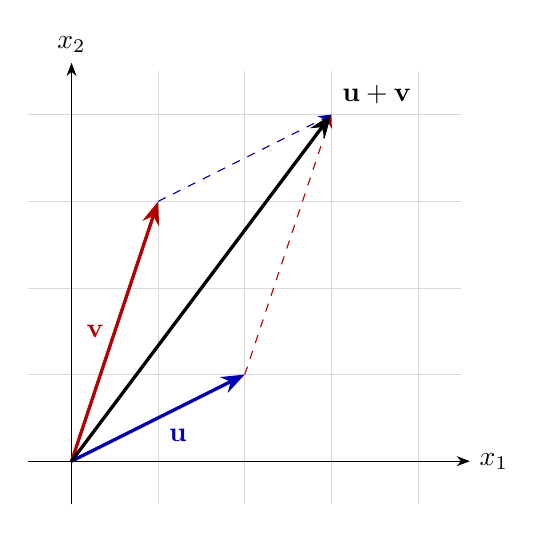
\begin{tikzpicture}[scale=1.1, >=Stealth]
  \draw[step=1, gray!30, very thin] (-0.5,-0.5) grid (4.5,4.5);
  \draw[->] (-0.5,0) -- (4.6,0) node[right] {$x_1$};
  \draw[->] (0,-0.5) -- (0,4.6) node[above] {$x_2$};
  \draw[->, very thick, blue!70!black] (0,0) -- (2,1) node[midway, below right] {$\mathbf{u}$};
  \draw[->, very thick, red!70!black] (0,0) -- (1,3) node[midway, left] {$\mathbf{v}$};
  \draw[->, dashed, red!70!black] (2,1) -- (3,4);
  \draw[->, dashed, blue!70!black] (1,3) -- (3,4);
  \draw[->, very thick] (0,0) -- (3,4) node[above right] {$\mathbf{u}+\mathbf{v}$};
\end{tikzpicture}
\end{center}

\begin{definition}
The \emph{span} of $\mathbf{v}_1,\dots,\mathbf{v}_p$ is the set of all linear
combinations $c_1\mathbf{v}_1 + \dots + c_p\mathbf{v}_p$. The vectors are
\emph{linearly independent} when $c_1\mathbf{v}_1 + \dots + c_p\mathbf{v}_p = \mathbf{0}$
only for $c_1 = \dots = c_p = 0$.
\end{definition}

\textbf{Check:} put the vectors as columns of $A$ and row reduce. They are
independent exactly when every column has a pivot.

\section{Matrices and row reduction}

Solve $A\mathbf{x} = \mathbf{b}$ by row reducing the augmented matrix:
\[
\left[\begin{array}{ccc|c}
1 & 2 & -1 & 3 \\
2 & 5 & 1 & 8 \\
-1 & -1 & 4 & 1
\end{array}\right]
\sim
\left[\begin{array}{ccc|c}
1 & 0 & 0 & 2 \\
0 & 1 & 0 & 1 \\
0 & 0 & 1 & 1
\end{array}\right],
\qquad
\mathbf{x} = \begin{bmatrix} 2 \\ 1 \\ 1 \end{bmatrix}.
\]

\begin{center}
\begin{tabular}{@{}lll@{}}
\toprule
Row operation & Effect on $\det A$ & Example \\
\midrule
Swap two rows & changes the sign & $R_1 \leftrightarrow R_2$ \\
Scale a row by $k$ & multiplies by $k$ & $R_2 \to 3R_2$ \\
Add a multiple of a row & no change & $R_3 \to R_3 + 2R_1$ \\
\bottomrule
\end{tabular}
\end{center}

\begin{theorem}[Invertible matrix theorem, part]
For an $n\times n$ matrix $A$, these say the same thing: $A$ is invertible;
$\det A \neq 0$; $A\mathbf{x}=\mathbf{0}$ has only the trivial solution; the
columns of $A$ span $\mathbb{R}^n$; $0$ is not an eigenvalue of $A$.
\end{theorem}

\section{Linear transformations and determinants}

The matrix $A = \begin{bmatrix} 2 & 1 \\ 0 & 1 \end{bmatrix}$ sends the unit
square to a parallelogram whose area is $|\det A| = 2$.

\begin{center}
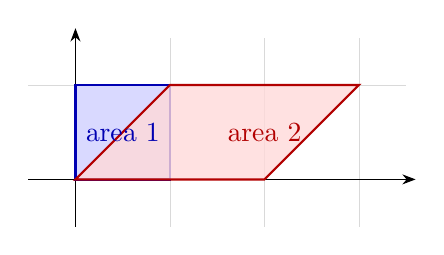
\begin{tikzpicture}[scale=1.2, >=Stealth]
  \draw[step=1, gray!30, very thin] (-0.5,-0.5) grid (3.5,1.5);
  \draw[->] (-0.5,0) -- (3.6,0);
  \draw[->] (0,-0.5) -- (0,1.6);
  \fill[blue!15] (0,0) -- (1,0) -- (1,1) -- (0,1) -- cycle;
  \draw[blue!70!black, thick] (0,0) -- (1,0) -- (1,1) -- (0,1) -- cycle;
  \fill[red!15, opacity=0.8] (0,0) -- (2,0) -- (3,1) -- (1,1) -- cycle;
  \draw[red!70!black, thick] (0,0) -- (2,0) -- (3,1) -- (1,1) -- cycle;
  \node[blue!70!black] at (0.5,0.5) {area 1};
  \node[red!70!black] at (2,0.5) {area 2};
\end{tikzpicture}
\end{center}

For a $2\times 2$ matrix, $\det\begin{bmatrix} a & b \\ c & d\end{bmatrix} = ad - bc$.
For larger ones, expand along a row or column with many zeros, or row reduce
to triangular form and multiply the diagonal.

\section{Eigenvalues and eigenvectors}

$\lambda$ is an eigenvalue of $A$ when $A\mathbf{x} = \lambda\mathbf{x}$ for some
$\mathbf{x}\neq\mathbf{0}$; find them as the roots of the characteristic
polynomial $\det(A - \lambda I) = 0$. For
$A = \begin{bmatrix} 4 & 1 \\ 2 & 3 \end{bmatrix}$:
\[
\det(A-\lambda I) = (4-\lambda)(3-\lambda) - 2 = \lambda^2 - 7\lambda + 10 = (\lambda-2)(\lambda-5).
\]

\begin{center}
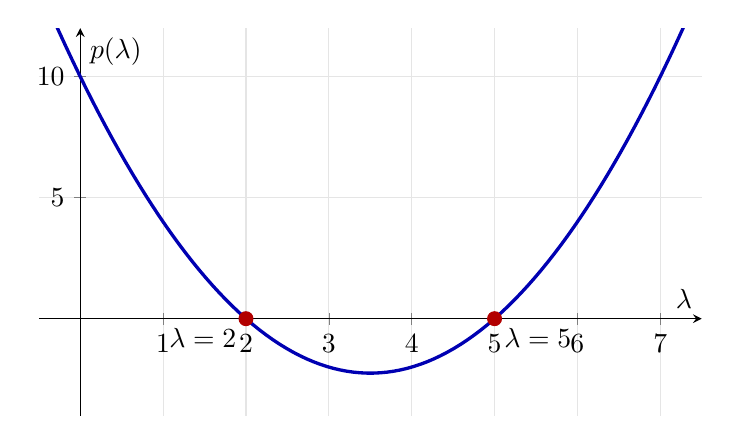
\begin{tikzpicture}
  \begin{axis}[
      width=10cm, height=6.5cm,
      axis lines=middle,
      xlabel={$\lambda$}, ylabel={$p(\lambda)$},
      xmin=-0.5, xmax=7.5, ymin=-4, ymax=12,
      grid=both, grid style={gray!20},
      samples=100, domain=-0.5:7.5]
    \addplot[very thick, blue!70!black] {x^2 - 7*x + 10};
    \addplot[only marks, mark=*, mark size=2.5pt, red!70!black] coordinates {(2,0) (5,0)};
    \node[below left] at (axis cs:2,0) {$\lambda=2$};
    \node[below right] at (axis cs:5,0) {$\lambda=5$};
  \end{axis}
\end{tikzpicture}
\end{center}

\section{Practice problems}

\begin{enumerate}[label=\arabic*.]
  \item Are $\begin{bmatrix}1\\2\\3\end{bmatrix}$, $\begin{bmatrix}4\\5\\6\end{bmatrix}$,
        $\begin{bmatrix}7\\8\\9\end{bmatrix}$ linearly independent? Explain with row reduction.
  \item Find $\det\begin{bmatrix} 1 & 2 & 0 \\ 3 & 1 & 4 \\ 0 & 2 & 1\end{bmatrix}$.
  \item Find the eigenvectors of $A = \begin{bmatrix} 4 & 1 \\ 2 & 3 \end{bmatrix}$ for $\lambda = 2$ and $\lambda = 5$.
  \item Describe what $\begin{bmatrix} 0 & -1 \\ 1 & 0\end{bmatrix}$ does to the plane, and give its determinant.
\end{enumerate}

\end{document}
